% !Mode:: "TeX:UTF-8" 

\BiChapter{数据分析及实验结果}{5}

\BiSection{生成式数据集分析}{}
数据集总共分为两部分\footnote{上述数据集统计信息截止于2024年5月6日,全部图像数据集均已开源:\\
\url{https://github.com/wty-yy/Clash-Royale-Detection-Dataset}\hfill}:
\begin{itemize}
  \item 生成式数据集切片:总计$154$个类别,待识别类别$150$个,总共包含$4654$个切片,
  在全部待识别类别的切片图像中,切片大小分布如图~\ref{fig-segment}~所示。
  \item 目标识别验证集:总计$6939$张人工标记的目标识别图像,包含$116878$个目标框,平均每张图片包含17个目标框,该数据集均为真实对局视频流逐帧标记得到,
  而模型训练所使用的完全是生成式数据集,所以该数据集可以做验证集使用。
\end{itemize}

\begin{figure}[htbp]
  \centering
  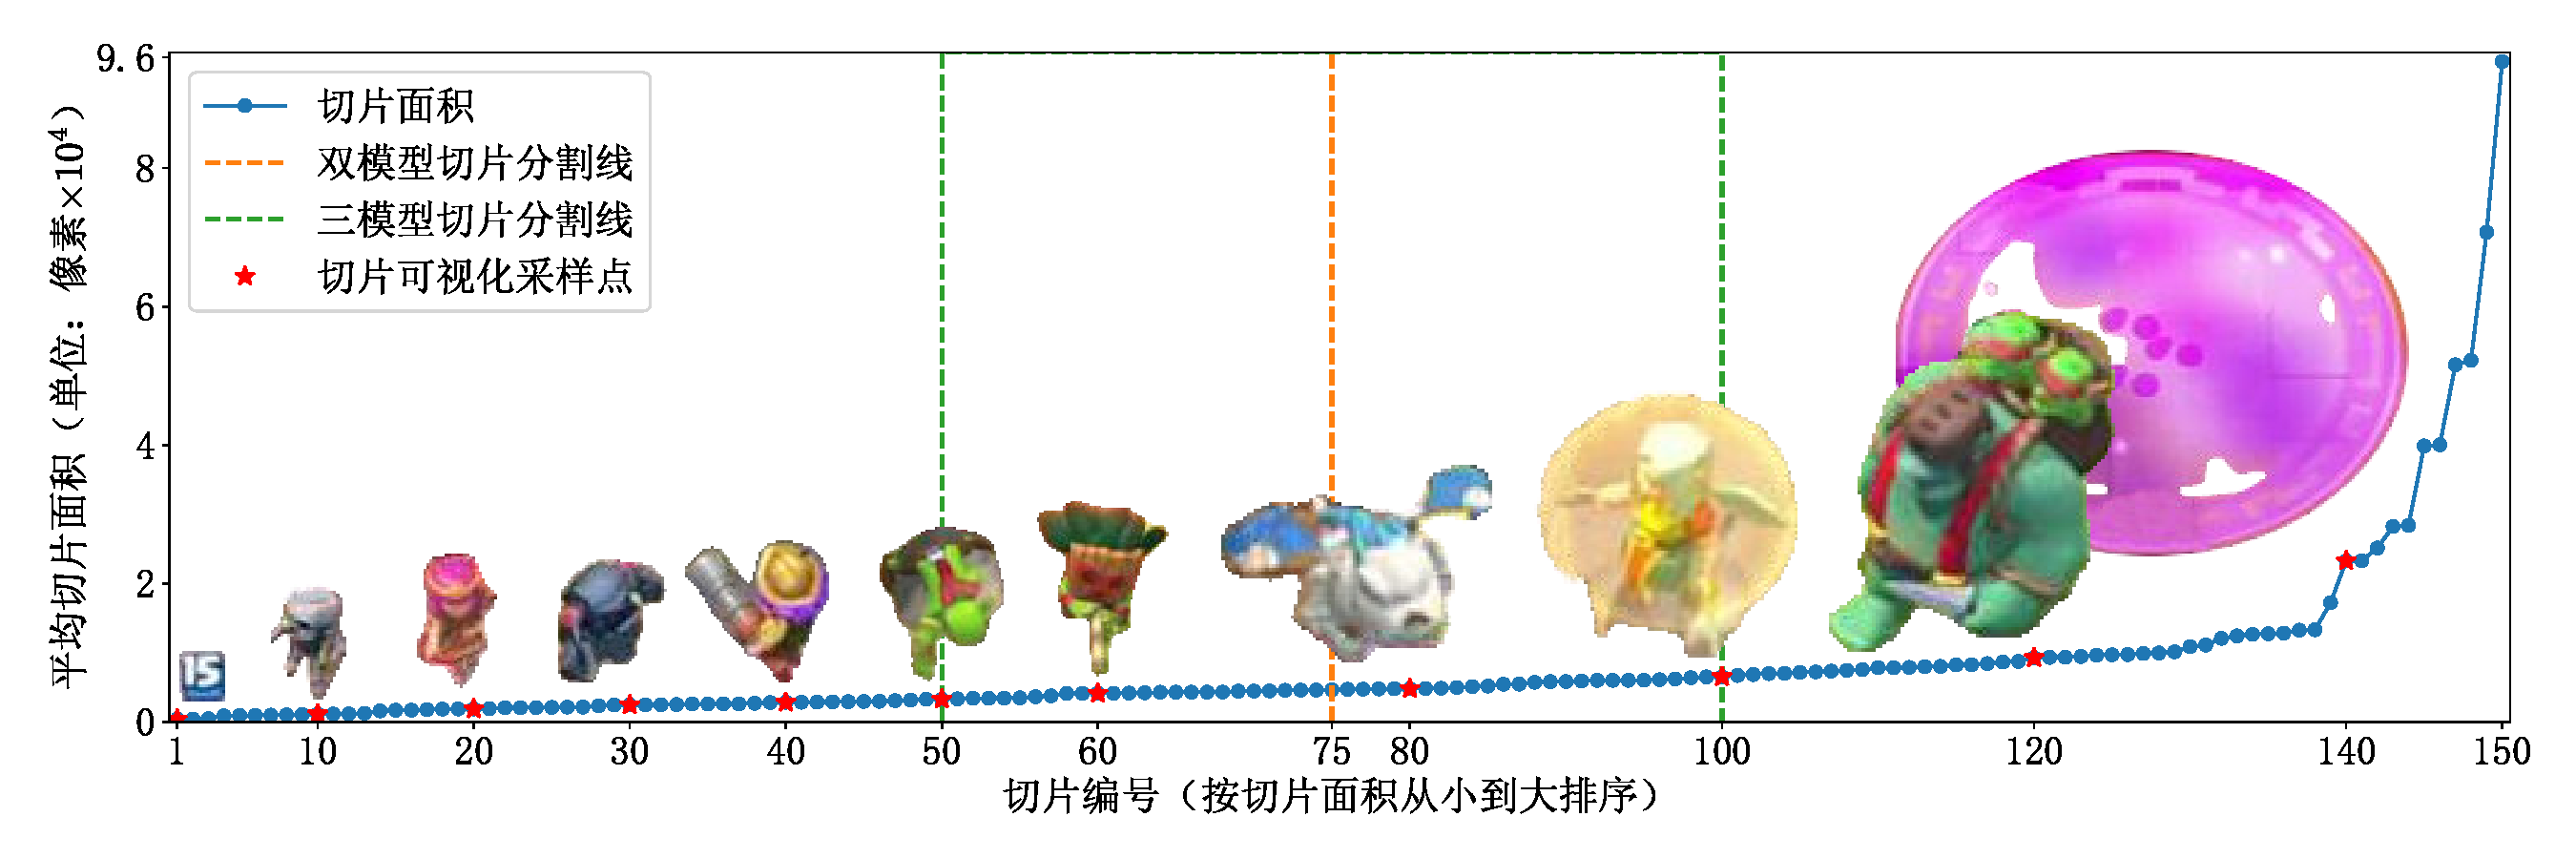
\includegraphics[width=\textwidth]{segment_size.pdf}
  \caption{将切片数据集全部切片按平均面积从小到大排序并编号,
  从中随机采样出部分切片进行可视化。
  分别以全体切片面积的二等分和三等分点,作为双模型和三模型的识别类别分割线。
  }
  \label{fig-segment}
\end{figure}

\BiSection{目标识别模型训练}{}
目标识别模型使用了自己实现的YOLOv5\footnote{复现YOLOv5代码:\url{https://github.com/wty-yy/KataCV/tree/master/katacv/yolov5}\hfill}
和重构后的YOLOv8的模型\footnote{YOLOv8重构内容:\url{https://github.com/wty-yy/KataCR/blob/master/asserts/yolov8_modify.md}\hfill},
每个训练集大小设置为$20000$,至多训练$80$个epoch收敛。
数据增强使用了:HSV增强,图像旋转,横纵向随机平移,图像缩放,图像左右反转,具体参数见附录~\ref{table-app-aug}~。

实验结果\footnote{YOLOv5全部训练曲线:\url{https://wandb.ai/wty-yy/ClashRoyale}\\\makebox[2.4ex][]{}YOLOv8全部训练曲线:\url{https://wandb.ai/wty-yy/YOLOv8}}如表~\ref{tabel-yolo}~所示,表中具体内容解释如下:

1. 模型名称:编号后的字母表示模型大小,l,x分别对应大与特大型模型,
YOLOv8-l$\times n$表示使用$n$个YOLOv8-l模型,每个子模型分别识别图~\ref{fig-segment}~中分割线所划分区域中的切片类型,
最后将识别的预测框通过非最大值抑制(Non-Maximum Suppression,NMS)进行筛选,NMS过程中IOU阈值设定为0.6。

2. 评测指标:表中mAP评测指标表示的是COCO\upcite{COCO}比赛提出的COCO mAP指标,即在10种不同IOU阈值下计算PR曲线下面积求平均得到,
AP50、P50和R50分别表示在判断正例的IOU阈值为$50\%$下的mAP、平均精度和平均召回率,。

3. 验证速度:模型预测时Batch大小设置为$1$,FPS为模型在GeForce RTX 4090下测试的验证速度,做验证机测试时置信度设置为$0.001$。
当对视频流数据进行预测时,将置信度改为$0.1$,并使用ByteTrack\upcite{ByteTrack}算法在目标追踪计算过程中对边界框进行筛选,
FPS(T)是在GeForce RTX 4060 Laptop下带有目标追踪的识别速度。

从实验结果可以看出,YOLOv8-l的双识别器对小目标的识别能力与三识别器效果基本一致,并远高出非组合式的识别器,
其原因可能在于$150$个预测类别大小远超模型的识别能力范围,
最大目标与最小目标的边界框大小差距甚远,又由于YOLOv8是无锚框识别头,
由于大目标易于识别,可能导致预测的目标框均偏大,所以多个识别器降低平均类别数能够有效对小目标进行识别。

\begin{table}[!h]
	\renewcommand{\arraystretch}{1.2}
	\centering\wuhao
	\caption{YOLO模型对比测试结果} \label{tabel-yolo} \vspace{2mm}
	\begin{tabularx}{\textwidth} { 
   >{\centering\arraybackslash}X 
   >{\centering\arraybackslash\hsize=.2\hsize}X
   >{\centering\arraybackslash\hsize=.2\hsize}X
   >{\centering\arraybackslash\hsize=.2\hsize}X
   >{\centering\arraybackslash\hsize=.2\hsize}X
   >{\centering\arraybackslash\hsize=.2\hsize}X
   >{\centering\arraybackslash\hsize=.3\hsize}X
   >{\centering\arraybackslash\hsize=.3\hsize}X
   >{\centering\arraybackslash\hsize=.9\hsize}X 
   >{\centering\arraybackslash\hsize=.7\hsize}X
  }
	% \toprule[1.5pt]
  \hline
  模型名称&mAP&AP50&P50&R50&FPS&FPS(T)&mAP(S)&检测器类别数&数据增强\\
  \hline
	% \midrule[1pt]
  YOLOv5-l&53.2&66.2&84.4&63.8&59&NA&NA&151&\\
  YOLOv8-x&67.7&83.1&\pmb{93.9}&68.3&68&31&39.8&160&\\
  YOLOv8-x&66.8&\pmb{85.3}&90.7&80.4&68&31&35.9&160&\checkmark\\
  YOLOv8-l~$\times 2$&67.4&84.3&89.5&79.8&34&18&43.9&85&\checkmark\\
  YOLOv8-l~$\times 3$&\pmb{68.8}&85.2&89.7&\pmb{80.9}&23&10&\pmb{48.3}&65&\checkmark\\
  \hline
	% \bottomrule[1.5pt]
	\end{tabularx}
\end{table}

\BiSection{决策模型训练}{}
本毕设基于第~\ref{chpt-perceptron}~章中介绍的感知融合技术,
手动构建了玩家与与游戏内置的$8000$分AI对局$105$回合的专家数据
\footnote{全部专家数据集均已开源:\url{https://github.com/wty-yy/Clash-Royale-Replay-Dataset}},
固定双方使用的卡组(具体卡组见附录~\ref{app-sec-desk}~),
数据集总计$113981$帧,动作帧占比$4.01\%$,重采样频次比率为$\frac{\text{动作帧}}{\text{非动作帧}}=24.92:1.04$,
平均动作延迟大小为$21.26$,最大间隔帧数阈值为$T_{delay}=20$(重采样细节见~\ref{sec-target})。
模型损失函数分为三个部分,由于均为离散动作,所以损失函数均使用目标动作均使用交叉熵损失(定义~\ref{def-cross-entropy}~),总损失函数如下
\begin{equation}
  \mathcal{L} =
  \sum_{\substack{i=1\\}}^N\left[a_i^{delay} < T_{delay}\right]\left[\mathcal{L}_{CE}(\hat{\bd{a}}_i^{pos}, \bd{a}_i^{pos})+
  \mathcal{L}_{CE}(\hat{a}_i^{select}, a_i^{select}) + 
  \mathcal{L}_{CE}(\hat{a}_i^{delay}, a_i^{delay})\right]
\end{equation}
其中$T_{delay},\bd{a}_i^{pos},a_i^{select},a_i^{delay}$分别为最大间隔帧数阈值、目标动作的部署坐标、手牌编号以及部署延迟,
注意每条轨迹下只考虑$\bd{a}_i^{delay} < T_{delay}$对应的梯度。

本文分别测试了下述模型参数:
\begin{enumerate}
  \item 不同的模型架构(架构设计见~\ref{sec-model}~),分别测试了StARformer和DT架构。
  \item 模型输入的轨迹步长记为$L$,测试了$L=30,50,100$的情况。
  \item 不同的预测目标(离散与连续预测见~\ref{sec-target}~)。
  \item 不同的手牌预测范围,默认预测当前手牌编号,也尝试了对当前牌库中全部手牌进行预测。
\end{enumerate}

本文使用了如下数据增强方式对模型进行训练:
\begin{itemize}
  \item 重采样:对稀疏的动作帧进行大量重采样,加快模型收敛,缓解离线数据集的长尾问题。
  \item 随机手牌重组:对当前输入轨迹中的全部手牌按照随机排列进行打乱,当预测当前手牌编号时,将动作对应的手牌也进行相应变换。
\end{itemize}

全部模型训练曲线均进行了上传\footnote{决策模型全部训练曲线:\url{https://wandb.ai/wty-yy/ClashRoyale\%20Policy}},
模型实时对局的验证结果总结于表\ref{table-model-eval}中,在实时对局的实现中包含以下细节:
\begin{itemize}
  \item 动作执行:对于连续动作预测模型中,由于感知识别中存在延迟,当预测动作延迟在$8$帧以内就会立刻执行动作,
  并且为了避免总圣水溢出导致的惩罚奖励,每当总圣水达到$10$时就直接下出当前预测的卡牌。
  \item 无效动作跳过:若模型预测出的卡牌所需圣水超出了当前总圣水量或当前动作执行的卡牌位为空。
\end{itemize}

\begin{table}[!h]
	\renewcommand{\arraystretch}{1.2}
	\centering\small
  %\wuhao
	\caption{决策模型对比}\label{table-model-eval}\vspace{2mm}
	\begin{tabularx}{\textwidth} { 
   >{\centering\arraybackslash\hsize=1.4\hsize}X 
   >{\centering\arraybackslash\hsize=0.6\hsize}X 
   >{\centering\arraybackslash}X 
   >{\centering\arraybackslash}X
   >{\centering\arraybackslash}X
   >{\centering\arraybackslash}X 
   >{\centering\arraybackslash}X 
   >{\centering\arraybackslash\hsize=.5\hsize}X
   }
	\toprule[1.5pt]
	模型框架&步长$L$&训练回合&总奖励&对局时长&动作数&胜率\\
	\midrule[1pt]
  DT-4L&50&8&$-5.7\pm 2.5$&$148.9\pm 33.6$&$128.7\pm 37.7$&$5\%$\\
  StARformer-2L&30&3&$-6.0\pm 2.3$&$135.0\pm 35.1$&$141.8\pm 57.9$&$5\%$\\
  StARformer-2L&50&8&$-6.2\pm 2.2$&$131.9\pm 44.3$&$195.3\pm 69.8$&$5\%$\\
  StARformer-2L&100&1&$-4.9\pm 2.8$&$150.2\pm 35.6$&$187.6\pm 48.2$&$0\%$\\
  StARformer-3L&30&4&$-5.1\pm 3.7$&$147.2\pm 37.4$&$190.8\pm 52.7$&\pmb{$10\%$}\\
  StARformer-3L&50&3&\pmb{$-4.7\pm 3.1$}&\pmb{$158.9\pm 27.7$}&\pmb{$207.8\pm 48.2$}&$5\%$\\
  StARformer-3L&100&5&$-6.1\pm 2.2$&$125.9\pm 37.8$&$144.6\pm 42.9$&$5\%$\\
  \makecell[c]{StARformer-3L\\(全卡牌预测)}&50&2&$-5.6\pm 2.1$&$150.2\pm 38.6$&$195.3\pm 69.8$&$0\%$\\
  \makecell[c]{StARformer-2L\\(离散动作预测)}&50&1&$-7.5\pm 0.8$&$123.1\pm 39.2$&$21.9\pm 9.4$&$0\%$\\
	\bottomrule[1.5pt]
	\end{tabularx}
\end{table}

表~\ref{table-model-eval}~中每个模型取前10个训练结果,将其每次与环境交互20个回合得到的最高奖励,
每列的含义分别为:
\begin{itemize}
  \item 步长$L$:为模型架构设计~\ref{sec-model-struct}~中的输入轨迹长度。
  \item 训练回合:前10个训练结果中,获得最高奖励所对应的回合数。
  \item 总奖励:按奖励公式~\ref{eq-reward}~进行累计得到的总奖励。
  \item 对局时长:统计每次对局的时长,单位秒。
  \item 动作数:统计每局智能体成功执行的动作数目。
  \item 胜率:按照~\ref{game-target}~中介绍的游戏目标,判定智能体的获胜概率。
\end{itemize}

图~\ref{fig-model-eval}~中展示了每种模型前10个训练结果曲线,从中可以看出,
本文将离散预测改为连续预测、StARformer架构从2L修改为3L的改动均能够显著提高模型性能,

\begin{figure}[htbp]
  \centering
  \subfigure[不同模型结构]{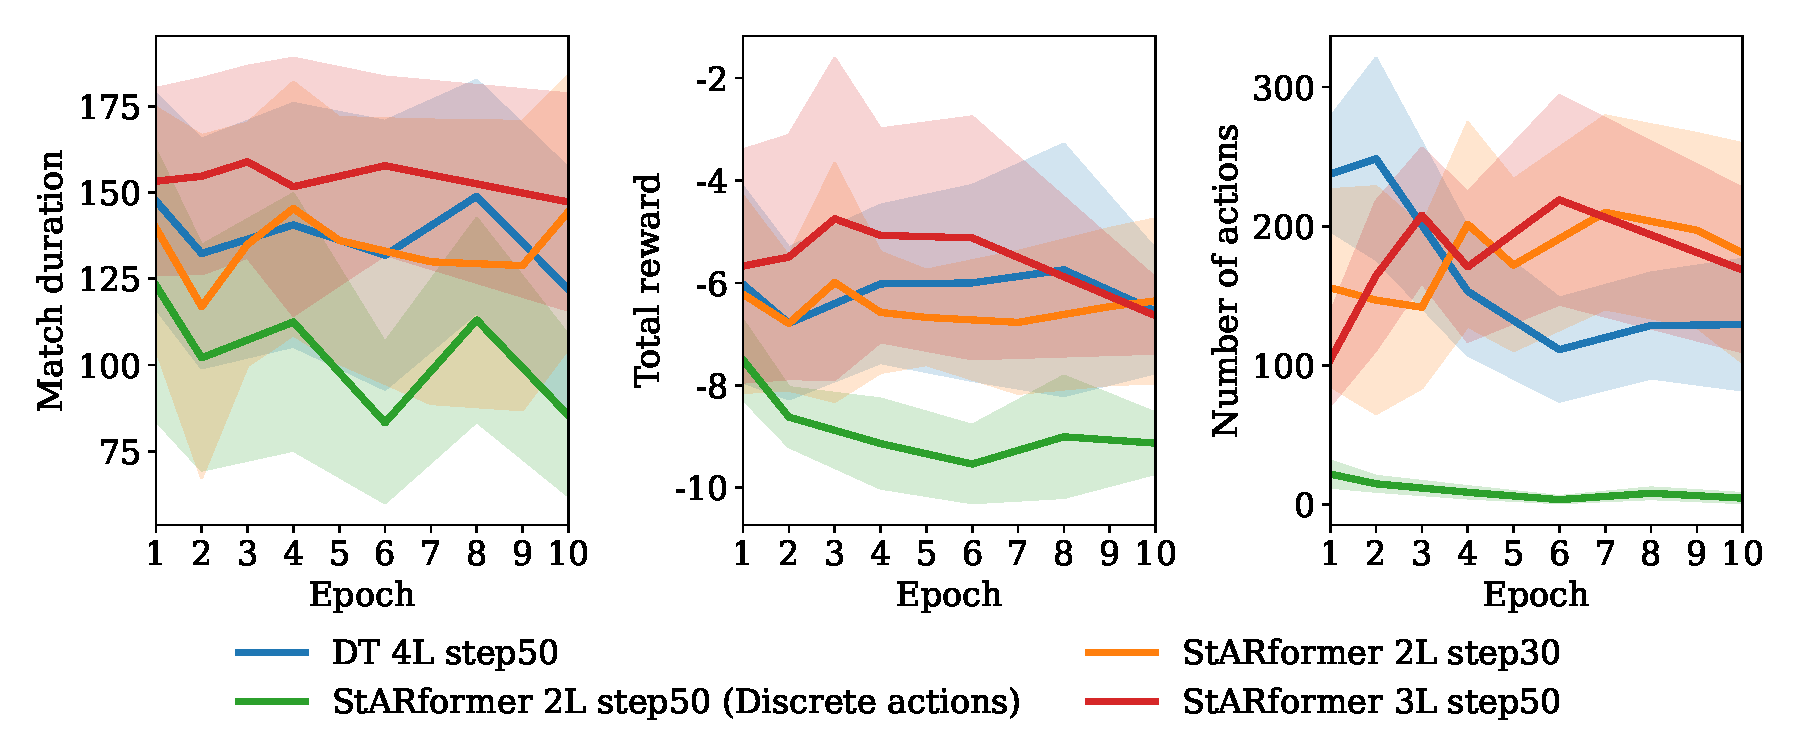
\includegraphics[width=\textwidth]{diff_model.pdf}}
  \subfigure[StARformer-3L采取不同轨迹长度]{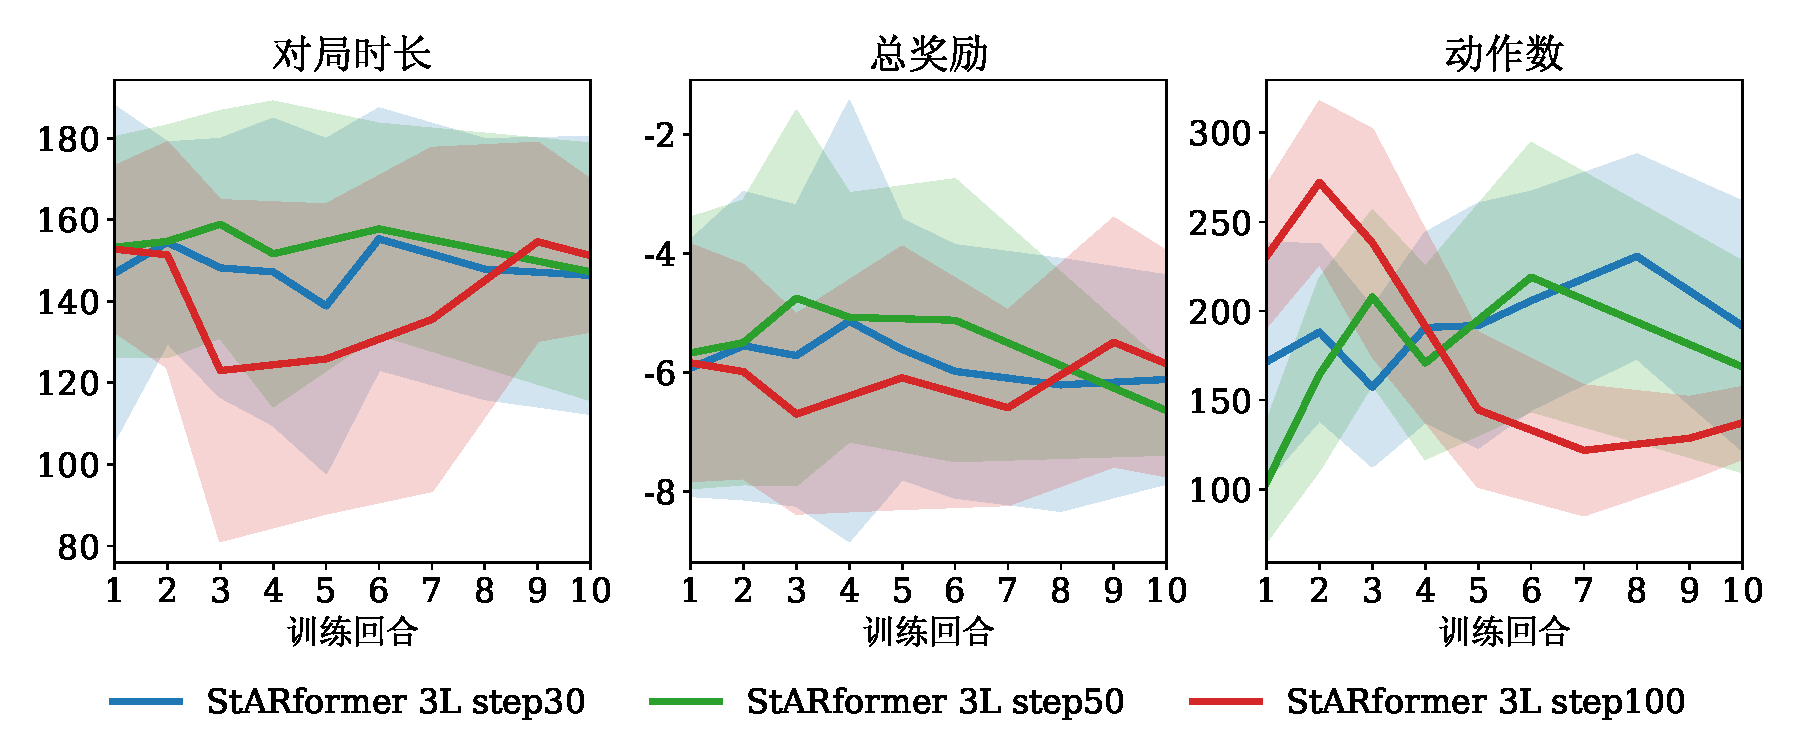
\includegraphics[width=\textwidth]{diff_3L_nstep.pdf}}
  \setlength{\abovecaptionskip}{0ex}  % 由于minted会增大图像与标题间距需要进行缩小
  \caption{模型验证曲线:展示了前10个训练结果,每回合模型在真实对局中的对局时间时长、总奖励和执行动作数,
  每次进行20次对局,实线为均值、虚影为标准差。}\label{fig-model-eval}
\end{figure}